% Esquemas de Recursos/2025-10-02.pdf, páginas 4 y 6.

% Una misma caja horizontal mantiene alineados los centros de ambos esquemas.
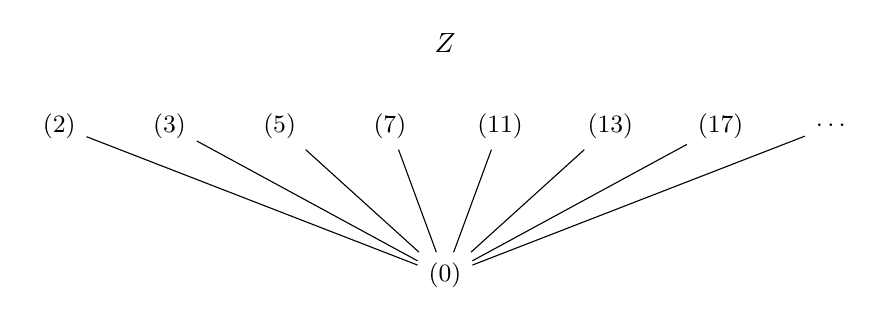
\begin{tikzpicture}[font=\small,inner sep=3pt,outer sep=1pt]
\useasboundingbox (-5.3,-.25) rectangle (5.3,3.15);
\node[font=\normalsize] at (0,2.95) {$\Spec\mathbb Z$};
\node (cero) at (0,0) {$(0)$};
\foreach \x/\p in {-4.9/2,-3.5/3,-2.1/5,-.7/7,.7/11,2.1/13,3.5/17}{%
  \node (p\p) at (\x,1.9) {$(\p)$};
  \draw (cero) -- (p\p);
}
\node (mas) at (4.9,1.9) {$\cdots$};
\draw (cero) -- (mas);
\end{tikzpicture}

\par\vspace{14pt}\noindent
\begin{tikzpicture}[font=\small,inner sep=3pt,outer sep=1pt]
\useasboundingbox (-5.3,-2.1) rectangle (5.3,4.15);
\node[font=\normalsize] at (0,3.9) {$\Spec\mathbb C[x]$};
\coordinate (O) at (0,-1.5);
\draw[dash dot] (-3.7,.6)--(2.8,.6)--(4.1,2.4)--(-2.4,2.4)--cycle;
\node[below=5pt] (zero) at (O) {$(0)$};
\foreach \name/\x/\y in {a/-2.8/1,b/-1.65/1.95,c/-.75/1.35,d/.8/1.95,e/2.15/1.3,f/3.1/1.95}{%
  \coordinate (\name) at (\x,\y);
  \pgfmathsetmacro{\fraccion}{2.1/(\y+1.5)}
  \path (O)--(\name) coordinate[pos=\fraccion] (corte);
  \draw (O)--(corte);
  \draw[dashed] (corte)--(\name);
  \fill (\name) circle (1.5pt);
}
\node[above left=2pt] at (c) {$0$};
\node[below left=2pt] at (d) {$i$};
\node[above right=2pt] at (e) {$1$};
\node at (-.75,2.85) {$(x)$};
\node at (.8,2.85) {$(x-i)$};
\node at (2.35,2.85) {$(x-1)$};
\end{tikzpicture}
